\documentclass[12pt,twoside,a4paper]{article}

\usepackage{polski}
\usepackage[utf8]{inputenc}
\usepackage{graphicx}
\usepackage{geometry}
\usepackage{fancyhdr}
\usepackage{amsthm}
\usepackage{url}
\usepackage{wrapfig}
\usepackage{float}
\usepackage{listings}
\usepackage{color}
\usepackage{xcolor}
\usepackage{natbib}

\floatstyle{ruled}

\lstset {
basicstyle=\scriptsize\ttfamily ,
numbers=left,
keywordstyle=\color{blue},
inputencoding=utf8,
literate={ą}{{\k{a}}}1
{Ą}{{\k{A}}}1
{ę}{{\k{e}}}1
{Ę}{{\k{E}}}1
{ó}{{\'o}}1
{Ó}{{\'O}}1
{ś}{{\'s}}1
{Ś}{{\'S}}1
{ł}{{\l{}}}1
{Ł}{{\L{}}}1
{ż}{{\.z}}1
{Ż}{{\.Z}}1
{ź}{{\'z}}1
{Ź}{{\'Z}}1
{ć}{{\'c}}1
{Ć}{{\'C}}1
{ń}{{\'n}}1
{Ń}{{\'N}}1,
}
\usepackage{caption}

\DeclareCaptionFont{white}{\color{white}}
\DeclareCaptionFormat{listing}{\colorbox{gray}{\parbox{\textwidth}{#1#2#3}}}
\captionsetup[lstlisting]{format=listing,labelfont=white,textfont=white}
\captionsetup[figure]{singlelinecheck=off,justification=raggedright}

\frenchspacing
\linespread{1.3}
%\geometry{verbose, a4paper, tmargin=2cm, bmargin=2cm,lmargin=2cm,rmargin=2cm}
%\geometry{verbose, a4paper, tmargin=2.5cm, bmargin=2.5cm,lmargin=3cm,rmargin=2cm}
\geometry{verbose, a4paper, tmargin=2cm, bmargin=2cm,lmargin=3cm,rmargin=2cm}


\pagestyle{fancy} %% deklarujemy styl "fancy"
\fancyhead{} \fancyfoot{} %% "zresetuj" zawartość pagin
\renewcommand{\sectionmark}[1]{\markright{\thesection\ #1}}
\fancyhead[LE,RO]{\normalfont \small \thepage}
\fancyhead[LO]{\normalfont \small \itshape \rightmark}
\fancyhead[RE]{\normalfont \small \itshape \rightmark}
\fancypagestyle{plain}{\fancyhead{}\renewcommand{\headrulewidth}{0pt}} %% ustaw paginy dla stylu plain

%\fancyhead{\chead{Wyższa Szkoła Informatyki Stosowanej i Zarządzania w Warszawie}}
%\pagestyle{fancy}

% title page

% koniec strona tytulowa
\newcommand{\HRule}{\rule{\linewidth}{0.1mm}}

\begin{document}
\begin{titlepage}

\begin{center}


% Upper part of the page
%\includegraphics[width=0.15\textwidth]{./logo}\\[1cm]    
\textsc{\Large Wyższa Szkoła Informatyki Stosowanej i Zarządzania}\\[0.1cm]
\textsc{pod auspicjami Polskiej Akademii Nauk}\\[0.1cm]
\textsc{\Large Wydział Informatyki}\\[0.1cm]
\textsc{\large Studia I stopnia }\\
\textsc{\large (inżynierskie)}\\[1.5cm]
\textsc{\LARGE PRACA DYPLOMOWA}\\[1.5cm]

\textsc{\LARGE Mariusz Skóra}\\[0.5cm]


% Title
\rule{\linewidth}{0.5mm} \\[0.9cm]
{ \huge \bfseries Projekt i implementacja systemu społecznościowego}\\[0.4cm]

\rule{\linewidth}{0.5mm} \\[1.5cm]

% Author and supervisor
\begin{minipage}{0.4\textwidth}
\begin{flushleft} \large

\end{flushleft}
\end{minipage}
\begin{minipage}{0.4\textwidth}
\begin{flushright} \large
\emph{Opiekun pracy:} \\
dr~Jan \textsc{Nowak}
\end{flushright}
\end{minipage}

\vfill

% Bottom of the page
{\large WARSZAWA, 2012}

\end{center}

\end{titlepage}

%Spis treści
\setcounter{page}{3}
%\begin{verse}
	\tableofcontents
%\end{verse}


\addcontentsline{toc}{section}{Słownik}
\thispagestyle{empty}
\section*{Słownik}\label{sec:slownik}

\begin{description}
\item \textbf{Literatura} \\
- literatura (bibliografia) znajduje się w pliku bibliografia.bib. Znajdują się tam pozycje wykorzystane w pracy. W dziale literatura pojawi się wpis dopiero wtedy, gdy w całej pracy wspomnimy o tej pozycji. Na przykład:
\cite[s.\pageref{sec:literatura}]{book:helloandroid}. Czasami trzeba kilka razy skompilować plik tex aby wyswietlił się numer i pozycja w literaturze

\item \textbf{Numeracja rysunków, tabel, listingów} \\
- każdy listing, tabela, rysunek musi być podpisany i odwoładnie do niego musi znajdować się w tekście przez referencje

\item \textbf{Obrazy} \\
- można wykorzystać obrazy umieszczone w wymaganiach. Wystarczy skopiować fragment kodu, podmienić ścieżkę do obrazku, zmienić label i poprawić podpis

\item \textbf{Referencje} \\
- referencje występują w tekscie tylko raz i zawsze na końcu zdania przed kropką. Referencja pojawia się tylko wtedy gdy po raz pierwszy padnie słowo, które wymaga referencji, na przykład \emph{Google} i \emph{Android} \cite[s.\pageref{sec:referencje}]{google,android}

\item \textbf{Wyliczenia} \\
- jednoroczne zaczynamy duża literą i kończymy kropką.

\end{description}



\newpage
\section*{Wstęp}
\addcontentsline{toc}{section}{Wstęp}
	% Wstep
\thispagestyle{empty}
Niniejszy dokument to szkielet pracy dyplomowej napisany w systemie \LaTeX.
Wstęp pracy dyplomowej powinien mieścić się na jednej stronie A4. Zawarty jest w nim krótki opis motywacji. 
Proszę skompilować cały plik zaczynając od START.TEX aby wykluczyć błędy kompilacji.
Najważniejsze:
\begin{itemize}
 \item każdy wyraz pochodzenia obcego, który nie jest polski lub nie jest słowem naturalnym oraz akronimy, czyli: \emph{IBM}, \emph{ID}, \emph{Python}, \emph{Microsoft} piszemy \emph{kursywą},
 \item elementy kodu aplikacji piszemy czcionką ze stałą odległością, tak zwaną typy \emph{monospace}. Przykład: \texttt{toJestMetoda} a \texttt{ToJestKlasa},
 \item dokument powinien być czytelny,
 \item pracę dyplomową piszemy bezosobowo,
 \item listowanie, czyli takie jak to, odzielamy przecinkami, 
 \item listowanie, czyli takie jak to, zawsze kończymy kropką.
\end{itemize}

INSTALACJA PAKIETÓW \LaTeX - \\
\begin{verbatim}
sudo apt-get install texlive-lang-polish install 
sudo apt-get install texlive-latex-extra install (312MB)
\end{verbatim}

Niniejszy dokument został przygotowany w programie KILE na systemie Ubuntu 12.04 LTS 64bit.\\
W razie problemów można kontaktować się na mój adres \emph{e-mail}: m.skora@gmail.com.


\newpage
\section{Cel pracy}
	\fancypagestyle{plain}
UUWAGA:
CELE PRACY to jeden z najważniejszych fragmentów pracy dyplomowej! W nim zawarte powinno być jakie cele student określił przed stworzeniem projektu dyplomowego. Recenzent pracy bada czy student zrealizował postawione CELE.
\\
Cele muszą być wymienione w punktach tak jak w przykładzie. Pamiętamy o referencjach.

W niniejszej pracy dyplomowej zostanie wyjaśnione w jaki sposób:
\begin{itemize}
\item zaprojektowano serwis społecznościowy (specyfikacja za pomocą diagramów \emph{UML}),
\item wykorzystano dostępne technologie (platforma \emph{PHP}, \emph{framework CakePHP} \cite[s.\pageref{sec:referencje}]{django}),
\item zaimplementowano aplikację (w językach \emph{PHP},
\item przetestowano system (wykorzystując dostępne narzędzia i skrypty testowe),
\item wdrożono system na serwerze \emph{Apache}\cite[s.\pageref{sec:referencje}]{apache}.
\end{itemize}
Dodatkowym celem jest wykazanie, że:
\begin{itemize}
\item można stworzyć serwis społecznościowy wykorzystując darmowe technologie typu \emph{Open Source} \cite[s.\pageref{sec:referencje}]{opensource}.
\end{itemize}
	
\newpage	
\section{Środowisko projektu}
	%srodowisko_projektu
Środowisko projektu to opis technologii jakie wykorzystujemy w budowie projektu dyplomowego. Po krótkim wstępie do rozdziału wymieniamy w punktach nasze środowisko. Pamiętamy o referencjach.\\

W programie wykorzystano:
\begin{enumerate}
 \item Język programowania - \emph{PHP}.
 \item Wykorzystany \emph{framework} - \emph{CakePHP}.
 \item System zarządzania bazami danych - \emph{PostgreSQL} \cite[s.\pageref{sec:referencje}]{postgresql}.
 \item Skrypty testujące - \emph{PHP Test Unit},
 \item Serwer \emph{Apache 2.2.20} (\emph{Ubuntu}),
 \item Edytor projektowy - \emph{NetBeans}, \emph{Vim} \cite[s.\pageref{sec:referencje}]{vim}.
\end{enumerate}

\newpage		
\section{Plan pracy}
	\begin{description}
\item[Rozdział 1.] 
Wyjaśniono cel pracy.
\item[Rozdział 2.] 
Omówiono środowisko projektu.
\item[Rozdział 4.] 
Określono wymagania oraz specyfikację projektu. Omówiono dlaczego podjęto się realizacji projektu aplikacji społecznościowej i co wchodzi w zakres pracy, 
i jaka jest charakterystyka podjętego przedsięwzięcia. W specyfikacji przedstawiono techniczne cechy projektu aplikacji.
\item[Rozdział 5.] 
Opisano wykorzystane środowisko projektowe.
\item[Rozdział 6.] 
Opisano wybrane moduły projektu. Omówiono komunikację między modułami w projekcie aplikacji internetowej.
\item[Rozdział 7.] 
Przedstawiono implementację systemu. Omówiono bezpieczeństwo.
\item[Rozdział 8.] 
Przedstawiono przypadki testowe dla testów jednostkowych, funkcjonalnych i integracyjnych.
\item[Rozdział 9.] 
Omówiono wdrożenie aplikacji webowej na serwerze \emph{Apache}.
\item[Rozdział 10.] 
Zamieszczono wnioski z tworzenia projektu.
\item[Rozdział 11.] 
Streszczono pracę w języku polskim i angielskim.
\end{description}
	% wymagania do projektu
\section{Wymagania do projektu}	
Poniżej znajduje się rysunek o numerze - \ref{rys:usecase2}. Numer został wygenerowany dynamicznie.
\begin{figure}[h!]
	\centering
	\HRule\\[1.5em]
		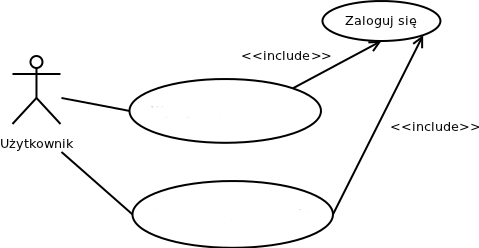
\includegraphics[width=0.5\textwidth]{img/usecase2.png}
	\\[0.3em]\HRule
	\captionof{figure}{Diagram przypadków użycia}
	\label{rys:usecase2}
\end{figure}

Mauris posuere euismod blandit. Mauris sapien ante, venenatis eget accumsan eget, lacinia at libero. Proin eget dui eros, at accumsan tortor. Aliquam sed quam libero, ac feugiat sem. Proin quis accumsan odio. Quisque posuere sollicitudin tellus, et rhoncus ipsum egestas sed. Cras nisl libero, condimentum nec porta vitae, faucibus vel purus. Pellentesque eget lorem quis elit iaculis ultricies. Fusce convallis venenatis augue, id consequat augue egestas vitae. Donec a lacus felis, consectetur tristique nibh. Sed vestibulum lectus in ipsum tincidunt fringilla. Cras sit amet consectetur nibh. Vestibulum sed est odio. 

Duis nibh enim, pretium vitae varius eget, mattis sed purus. Morbi tempor faucibus nisi at mattis. Phasellus aliquet ultrices diam, malesuada adipiscing elit iaculis quis. Fusce vel diam sit amet ligula sagittis vulputate volutpat ut dui. Maecenas cursus, turpis quis sagittis scelerisque, tortor tellus vulputate nibh, sed hendrerit nisi nisi et lacus. Suspendisse nec nisi felis. Cum sociis natoque penatibus et magnis dis parturient montes, nascetur ridiculus mus. 

Curabitur a nisi felis. Praesent tristique placerat malesuada. Nunc interdum lobortis accumsan. Lorem ipsum dolor sit amet, consectetur adipiscing elit. Nulla in sapien magna, at porttitor lorem. Vivamus condimentum convallis risus eget tincidunt. Vestibulum in condimentum magna. 

Sed quis purus est, at lobortis est. Maecenas condimentum lectus quis lectus scelerisque tristique. Sed sodales nisi in nisl tincidunt vel pretium justo hendrerit. Nullam sed ligula accumsan orci porta porttitor vitae quis lorem. Aliquam semper adipiscing tristique. Pellentesque consequat dapibus lectus vel vulputate. Proin vel ipsum massa. Vivamus suscipit, nulla ut accumsan vulputate, elit sapien hendrerit quam, at blandit odio lectus ac odio. Integer auctor, nunc vel porttitor lacinia, enim nibh faucibus nibh, a hendrerit libero dolor ut libero. 

\begin{figure}[h!]
	\centering
	\HRule\\[1.5em]
		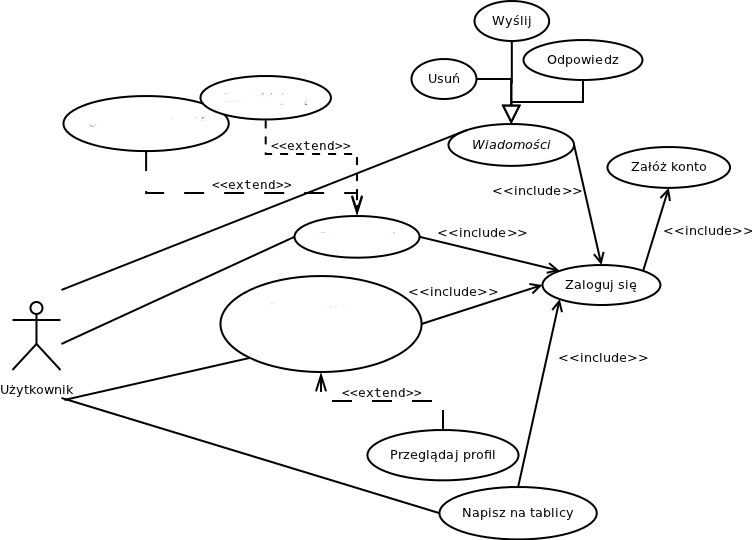
\includegraphics[width=0.8\textwidth]{img/usecase1.png}
	\\[0.3em]\HRule
	\captionof{figure}{Diagram przypadków użycia dla aplikacji internetowej}
	\label{rys:usecase1}
\end{figure}
\begin{figure}[h!]
	\centering
	\HRule\\[1.5em]
		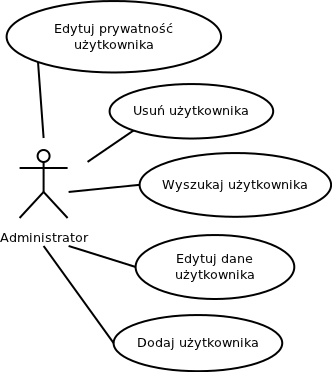
\includegraphics[width=0.4\textwidth]{img/usecase3.png}
        \\[0.3em]\HRule
	\captionof{figure}{Diagram przypadków użycia}
	\label{rys:usecase3}
\end{figure}


	% 2.1 Specyfikacja
\subsection{Specyfikacja}
W tym rozdziale musimy opisać specyfikację projektu. Omawiamy założenia projektowe, ograniczenia i problemy.



\newpage
\section{Architektura aplikacji}
	%architektura
Quisque metus odio, gravida non consequat at, consectetur sodales diam. Duis dignissim lacus et felis feugiat eget hendrerit ante dapibus. Phasellus tempus gravida purus vitae facilisis. Aliquam erat volutpat. Mauris non nisl magna. Sed nec enim nec tellus pellentesque pharetra in sit amet nunc. Ut ullamcorper, ipsum sit amet sodales commodo, nisl lectus dictum magna, porta pretium dui turpis a tortor. Quisque massa sapien, convallis ut viverra vitae, condimentum quis nisi. Nullam id arcu aliquam massa auctor ornare. Cras vestibulum justo sed elit vestibulum eu suscipit massa mattis. Sed posuere euismod nisi, sit amet lobortis ligula tempor quis. Donec in enim vel dui hendrerit elementum. Nulla eget nunc nisl, vel hendrerit risus:
\begin{itemize}
 \item posuere euismod nis,
 \item convallis ut viverra vitae, condime,
 \item nec enim nec tellus pellentesque. 
\end{itemize}
Nunc mauris libero, pulvinar eget ornare eget, sodales eget est. Nunc eget viverra diam. Curabitur sit amet urna sed dolor porttitor tincidunt at nec ante. Phasellus justo mauris, dapibus sed vehicula quis, venenatis at risus. Donec nec turpis nulla, ut porta libero. Maecenas eget mi augue. Donec convallis leo vitae purus hendrerit scelerisque. Mauris eros tellus, facilisis adipiscing semper a, vestibulum non tortor. Donec porta, justo quis ultricies faucibus, ligula odio elementum lorem, vitae molestie elit sem id dolor. Aliquam neque mi, sollicitudin et iaculis nec, laoreet eu sapien. Praesent pellentesque malesuada luctus. Fusce quis quam odio, et sodales massa. Nunc molestie nisl a quam hendrerit quis egestas urna commodo. Sed at blandit nulla. Duis pharetra egestas quam vel laoreet. Proin lacus justo, lacinia at rhoncus in, gravida vitae ipsum. 
	\subsection{Język PHP}
		%architektura-python
\emph{PHP} to skryptowy język programowania.
		\subsubsection{Framework CakePHP}
		\subsubsection{Wzorzec projektowy MVC}
	
	\subsection{Wykorzystane technologie}
		\subsubsection{PostgreSQL}
			%architektura-postgresql
To relacyjna, wydajna baza danych, początkowo rozwijana na Uniwersytecie Kalifornijskim w \emph{Berkeley} pod nazwą \emph{Ingres}. Później, aby uzgodnić zgodność ze standardem \emph{SQL}, zmieniono nazwę na \emph{PostgreSQL} (czasami nazywana również \emph{Postgres}). Wspomniany system baz danych obok innych darmowych rozwiązań takich jak \emph{MySQL} czy \emph{Firebird} wyróżnia się wysoką wydajnością oraz możliwościami jakie oferuje \cite[s.\pageref{sec:referencje}]{mysql,firebird}. Jednym z atutów \emph{Postres} jest możliwość pisania własnych poleceń składowanych w różnych językach programowania. Podobne rozwiązanie stosuje komercyjny \emph{Oracle}, gdzie można projektować funkcje przy pomocy \emph{PL/SQL}, a od wersji 8i również w języku \emph{Java} \cite[s.\pageref{sec:referencje}]{oracle}.

\newpage
\section{Opis modułów i komunikacja}
	%komunikacja
Jakiś wstęp
	\subsection{Diagramy klas}\label{kom-diagram-klas}	
		%komunikacja-diagram-klas



	\subsection{Aplikacja internetowa}

	\subsection{Edycja profilu}
		
	\subsection{Nawiązane znajomości}
	
	\subsection{Ochrona prywatności danych osobowych}
		
	\subsection{Administracja systemem}

\newpage
\section{Implementacja}\label{sec:implementacja}
	%implementacja
Jakiś wstęp\\

Dział implementacja nie powinien być zbytnio obszerny. Nie wolno wrzucać kodu całej aplikacji, ponieważ taka praca będzie źle oceniona. W tym dziale prezentujemy tylko taki kod jaki chcemy zaprezentować. Możemy na przykład wybrać sobie pewną ścieżkę w naszym programie i opisać ją tutaj za pomocą kodu. Należy czytelnie i logicznie opisać klasy, które są szczególne i ważne w drodze do realizacji jakiegoś zadania (żadania).

W tym dziale zostawiłem jeden rozdział, aby służył jako przykład.
	\subsection{Logowanie i rejestracja}
	  %implementacja-logirej
Implementacja logowania i rejestracji użytkowników to pierwsze zadanie zrealizowane podczas pisania projektu. W trakcie poszerzania możliwości serwisu, prezentowany kod często ulegał refaktoryzacji. Poniższy rozdział prezentuje ostateczną wersję kodu modułu rejestracji i logowania.

Pierwsza prezentowana funkcjonalność została napisana w języku \emph{Python} z zastosowaniem \emph{frameworka Django}, czyli tak jak większość opisywanej aplikacji. Mając na uwadzę stosowany wzorzec architektoniczny \emph{MVC}, w pierwszej kolejności zaprezentowany będzie model, a po nim logika biznesowa.

Najważniejszy model aplikacji, a zarazem profil użytkownika to klasa \texttt{UserProfile} (listing \ref{kod:UserProfile}).\\

\lstinputlisting[
  label=kod:UserProfile, 
  caption=Klasa modelu UserProfile]
  {src/UserProfile.py}

\vspace{1em}
Zaprezentowany kod ma swoje przełożenie na budowę tabel w bazie danych. \emph{Django} wykorzystuje modele po ich napisaniu do stworzenia tabel o takiej samej nazwie jak nazwa klasy modelu poprzedzona nazwą aplikacji. Parametry klasy \texttt{UserProfile} to kolumny tabeli.

Komentarza wymaga parametr \texttt{user}, \texttt{friends}
oraz 
\texttt{privacy}. 
Są to odwołania do kluczy obcych innych tabel utworzonych przez inne modele \emph{Django}. Parametr \texttt{user} to obiekt klasy wbudowanej \texttt{User}. Jest używany wszędzie tam gdzie wymagany jest obiekt użytkownika lub \emph{ID} encji w bazie danych. Parametr \texttt{friends} jest referencją do innej tabeli, utworzonej podczas tworzenia tabeli dla modelu \texttt{UserProfile}. Przechowuje ona relacje zawartej znajomości między użytkownikami serwisu. I ostatni parametr - \texttt{privacy} to referencja do klasy \texttt{UserPrivacy}, która odpowiada za prywatność użytkowników (listing \ref{kod:UserPrivacy}).\\

\lstinputlisting[
  label=kod:UserPrivacy, 
  caption=Klasa modelu UserPrivacy]{src/UserPrivacy.py}

\vspace{1em}
Za logikę aplikacji odpowiadają widoki. Poniżej prezentacja kodu aplikacji \texttt{accounts}, który realizuje rejestrowanie użytkowników (listing \ref{kod:register}). \\

\vspace{1em}
Metoda \texttt{register} to zwykła funkcja napisana w języku \emph{Python}. Przyjmuje ona tylko jeden parametr, którym jest żądanie (\texttt{request}) przesłane przez użytkownika. Jest to obiekt klasy \texttt{HttpRequest}, który przechowuje dość sporo informacji. Najważniejsza dla funkcji jest tablica \texttt{POST}, która przechowue dane wpisane do formularza. 
Za formularz rejestracji odpowiada klasa \texttt{RegisterForm} (listing \ref{kod:RegisterForm}).\\

\lstinputlisting[label=kod:RegisterForm, caption=Formularz rejestracji nowego użytkownika]{src/RegisterForm.py}

\vspace{1em}
Formularz \texttt{RegisterForm} posiada cztery parametry, które są obiektami klas wbudowanych w \emph{Django}. Sam formularz to również klasa i dziedziczy po głównej klasie \texttt{Form} z pakietu \texttt{django.forms}. Dzięki generalizacji, klasa formularza ma dostęp do trzech niezbędnych metod - \texttt{is\_valid}, \texttt{clean} oraz \texttt{save}. Pierwsza jest używana w funkcji \texttt{register} z poprzedniego kodu. Wywołuje ona metodę \texttt{clean} w klasie \texttt{Form}, która weryfikuje poprawność wypełnionego formularza i zwraca błąd, gdy formularz jest źle wypełniony. Metodę tą można nadpisać i dostosować do własnych wymagań, jednak w tej klasie wykorzystano tylko \texttt{is\_valid}, która zwraca \texttt{True} lub \texttt{False}.

Kolejna metoda - \texttt{save} - dodatkowo waliduje poprawność wprowadzonych danych, w sposób wymagany do poprawnego działania serwisu. Jeżeli weryfikacja napotka błąd, do widoku zostanie zwrócony \emph{False}, a na stronie zostanie wyświetlony odpowiedni komunikat. Jeżeli weryfikacja nie napotka żadnych problemów, zostaje utworzone nowe konto użytkownika, nowy profil oraz prywatny katalog na dysku serwera.

Pola formularza będą wyświetlone na stronie, bez znaczenia na wynik walidacji danych. Funkcja widoku zawsze tworzy instancję formularza, która jest zwracana jako parametr do szablonu \emph{template} \texttt{register.html}. Tam traktowany jest jak obiekt w specjalnym języku szablonów \emph{Django}. Na przykład wywołanie \texttt{\{\{form.email\}\}} zwróci na stronie formularz \emph{input} dla pola \emph{e\-mail}.

W kolejnej części znajduje się opis kodu odpowiedzialnego za logowanie użytkownika. W tym przypadku zaprezentowany zostanie wyłącznie kod logiki, ponieważ część modelu jest taka sama jak w przypadku rejestracji. Poniżej znajduje się kod widoku - funkcja \texttt{log\_in} z widoku aplikacji \texttt{accounts} (listing \ref{kod:log_in}).\\

\lstinputlisting[label=kod:log_in, caption=Funkcja logowania]{src/log_in.py}

\vspace{1em}
W tym przypadku, weryfikacja danych wymaganych do poprawnego działania aplikacji realizowana jest bezpośrednio po stronie widoku. Funkcja wywołuje formularz \texttt{LoginForm} (listing \ref{kod:LoginForm}).\\

\lstinputlisting[label=kod:LoginForm, caption=Formularz logowania]{src/LoginForm.py}

\vspace{1em}
Rolę jaką pełni funkcja widoku to przede wszystkim dopisywanie do obiektu \texttt{messages} wiadomości, które wyświetlone zostaną na stronie osoby wywołującej stronę logowania. Obiekt \texttt{messages} to element \emph{frameworka} o tej samej nazwie, który jest częścią \emph{Django}. Jego działanie jest proste i w zaprojektowanej pracy, realizuje przesyłanie wiadomości do użytkownika, które wyświetlone będą na stronie.

Po przeprowadzonej weryfikacji, w odpowiedzi zostanie zwrócony obiekt formularza do parametru \texttt{form}, uzupełniony o wiadomość w obiekcie \texttt{messages} - obiekt ten zwrócony jest do żadania w lini 33. 

Implementacja modułu logowania i rejestracji może z początku wyglądać dziwnie, mając w pamięci standardowe podejście do tworzenia i wyświetlania formularzy na stronie internetowej, na przykład w języku \emph{PHP}. Formularze \emph{Django} mają być przede wszystkim tak napisane, aby ich kod nie był powtarzany (zgodnie z zasadą \emph{DRY}) i po krótkiej analizie kodu, można dojść do wniosku, że framework robi to w sposób czytelniejszy. Dodatkowo \emph{Django} wyposarza programistę w dodatkowe narzędzia wspomagające walidację i prezentację danych na stronie.

Możliwość logowania na serwerze została zaimplementowana także w aplikacji na system \emph{Android}. Poniżej znajduje się kod klasy \texttt{Main}, gdzie realizowana jest podstawowa logika programu na platformie \emph{Android}.
Klasa \texttt{Main} posiada klasy \texttt{User} oraz \texttt{Geolocation} (listing \ref{kod:android-main}). Dziedziczy po głównej klasie \emph{Android} - \texttt{Activity} i implementuje interfejs \texttt{OnClickListener} udostępniający metodę \texttt{onClick} wywoływaną gdy dotknięty zostanie przycisk \texttt{loginButton}. Logika tej klasy realizowana jest w metodzie \texttt{onClick}, gdzie ładowane są ustawienia oraz uruchamiane jest logowanie do serwera.\\

\lstinputlisting[label=kod:android-main, caption=Klasa Main aplikacji \emph{Android}]{src/android-main.java}

\vspace{1em}
Metoda \texttt{onClick} tworzy obiekt klasy \texttt{User} o nazwie \texttt{user}, której konstruktor przyjmuje dwa parametry - \emph{e\-mail} oraz hasło pobrane z konfiguracji \texttt{preferences}. Następnie dla obiektu \texttt{user} wywołana zostaje metoda \texttt{tryLogin}, która loguje użytkownika na serwerze. W odpowiedzi aplikacja otrzyma kod \emph{200} albo \emph{401}.

Logowanie po stronie serwera realizuje funkcja \texttt{mlogin} z widoku aplikacji \texttt{mobile}. Jest ona podobna do funkcji \texttt{log\_in}, z tą różnicą, że \texttt{mlogin} przyjmuje dane w formacie \emph{JSON}. Po odczytaniu ich, następuje logowanie na serwerze lub zostanie zwrócony bład w razie niepowodzenia. Poniżej znajduje się kod funkcji \texttt{mlogin}.\\

\vspace{1em}
W przypadku \texttt{mlogin}, funkcja wykorzystuje formularz \texttt{LoginForm} z aplikacji \texttt{accounts}. Dane \emph{JSON} odczytane z przesłanego żądania \emph{HTTP} są przekazane do konstruktora klasy \texttt{LoginForm}. Jeżeli przesłane są niepoprawne, zwrócony zostanie status \emph{401}. Zaletą wykorzystania wcześniej napisanego formularza, jest wykorzystanie metody \texttt{clean}, która waliduje przesłane dane i zabezpiecza serwer przed niebezpiecznymi atakami.

Logowanie w serwisie ze strony aplikacji na platformę \emph{Android} i wewnątrz serwisu zostało zaprezentowane. Prezentowany kod realizuje swoje zadanie tak jak projektowano. Walidacja danych jest wykonywana poprawnie, a szczegóły walidacji oraz przyjęte przypadki testowe będą prezentowane w dziale \ref{sec:testy}.

	\subsection{Edycja profilu}
\newpage	
\section{Testy}\label{sec:testy}
  %testy
Wstęp na początku. Należy wyjaśnić dlaczego trzeba testować i co zostało w programie przetestowane. Można opisać jakieś założenia przed testowaniem. Ważne jest środowisko testowania, które w tym dziale należy zaprezentować.


	\subsection{Przypadki testowe dla testów jednostkowych}\label{sec:przypadki_testowe}
	\subsection{Testy funkcjonalne i integracyjne}\label{sec:testy_funkcjonalne}
	\subsection{Testy akceptacyjne}
	\subsection{Wnioski z testów}\label{sec:testy_wnioski}
\newpage	
\section{Wdrożenie aplikacji}
	\subsection{Instalacja aplikacji na serwerze Apache}
\newpage	
\section{Zakończenie}
  %zakonczenie
Na podstawie zakończenia recenzent pracy wystawia opinię na temat studenta. Zakończenie jest napisane w czasie przeszłym (zrobiono, napisano, przetestowano) i musi prezentować rozwiązanie postawionych wcześniej celów. Zazwyczaj jeden akapit w zakończeniu odpowiada jednemu punktowi w celach pracy.

  \subsection{Wnioski}

  \subsection{Dalszy rozwój aplikacji}


\newpage
\section{Streszczenie}

%referencje
%\bibliographystyle{abbrv}

\renewcommand*{\refname}{} % This will define heading of bibliography to be empty, so you can...
\section*{Referencje}\label{sec:referencje}     % ...place a normal section heading before the bibliography entries.
\addcontentsline{toc}{section}{Referencje}
\bibliographystyle{ieeetr}
\begin{thebibliography}{99}
\bibitem{iphone}
	\emph{iPhone} - Smartfon opracowany i wyprodukowany przez firmę \emph{Apple Inc.}. 
	\url{www.iphone.com}
\bibitem{apple}
	Apple Inc. - Amerykańska korporacja zajmująca się projektowaniem i produkcją elektroniki użytkowej, 
	oprogramowania i komputerów osobistych. Mieści się w \emph{Cupertino} w Kaliforni (USA). 
	\url{www.apple.com}
\bibitem{google}
	\emph{Google Inc.} - Amerykańskie przedsiębiorstwo z branży internetowej. Producent systemu operacyjnego \emph{Android}.
	\url{www.google.com}
\bibitem{android}
	\emph{Android} - System operacyjny dla urządzeń mobilnych.	
	\url{www.android.com}
\bibitem{python}
	\emph{Python} - Interpretatywny, obiektowy język programowania.
	\url{www.python.org}
\bibitem{java}
	\emph{Java} - obiektowy język programowania wysokiego poziomu.
	\url{http://www.java.com/en/java_in_action/}	
\bibitem{apache}
	\emph{Apache2} - Najpopularniejszy, otwarty serwer \emph{HTTP}.
	\url{http://httpd.apache.org/}
\bibitem{opensource}
	\emph{Open Source} - Ruch promujący otwarte oprogramowanie.
	\url{http://www.opensource.org/}
\bibitem{postgresql}
	\emph{PostgreSQL} - System zarządzania bazami danych \emph{PostgreSQL}.
	\url{www.postgresql.org}
\bibitem{modwsgi}
	\emph{MOD WSGI} - Adapter języka \emph{Python} dla serwera \emph{Apache}.
	\url{http://code.google.com/p/modwsgi/}
\bibitem{sublime_text}
        \emph{Sublime Text 2} - Edytor tekstu i kodu aplikacji
	\url{http://www.sublimetext.com/}
\bibitem{vim}
	\emph{VI Improved} - Wieloplatformowy edytor tekstowy należący do grupy wolnego oprogramowania o otwartym kodzie źródłowym.
	\url{http://www.vim.org/}
\bibitem{eclipse}
	\emph{Eclipse} - Środowisko programistyczne.
	\url{www.eclipse.org/}
\bibitem{android-sdk}
	\emph{Android SDK} - Narzędzia programistyczne, biblioteki, \emph{debugger} kodu, emulator i dokumentacja.
	\url{http://developer.android.com/sdk/index.html}
\bibitem{adb}
	\emph{Android Debug Bridge (ADB)} - Narzędzie wchodzące w skład \emph{Android SDK}, narzędzie lini poleceń typu klient-serwer pozwalające na komunikację z emulatorem urządzenia lub z urządzeniem z systemem operacyjnym \emph{Android}.
\bibitem{ubuntu1110}
	\emph{Linux Ubuntu 11.10} - System operacyjny typu \emph{Open Source}.
	 \url{www.ubuntu.com}
\bibitem{androidmarket}
	\emph{Android Market} - Internetowy sklep \emph{Google} z aplikacjami na urządzenia działające pod kontrolą systemu operacyjnego \emph{Android}.
	\url{http://market.android.com}	
\bibitem{wersje_android}
	\emph{Wersje platformy Android}\\
	\url{http://developer.android.com/resources/dashboard/platform-versions.html}	
\bibitem{google_maps}
	\emph{Google Maps} - Serwis internetowy umożliwiający wyszukiwanie obiektów, oglądanie map i zdjęć lotniczych z powierzchni Ziemi.
	\url{www.maps.google.pl}

\end{thebibliography}





\include{spis_rysunkow}

\include{spis_listingow}

\section*{Literatura}\label{sec:literatura}
\addcontentsline{toc}{section}{Literatura}
\bibliography{bibliografia}
\bibliographystyle{plain}

%\include{zalaczniki}


\end{document}
